\documentclass{article}
\usepackage[utf8]{inputenc}
\usepackage[italian]{babel}
\usepackage[a4paper, total={6in, 10in}]{geometry}
\usepackage{hyperref}
\usepackage{graphicx}
\graphicspath{ {./img/} }

\title{Relazione ingegneria - Monopoly 1}
\author {\textbf{Team Gang of Four 2}\\Acerbis Gianluca\\Canesi Gabriele\\Di Pierro Luca\\Fiorenza Gioele}
\date{\today}

\begin{document}

\maketitle

\section{Analisi}

\subsection{Premessa}
Essendo alcuni diagrammi particolarmente grandi, abbiamo preferito, per poter permettere la loro visione  renderli consultabili attraverso il browser.
Cliccando sulle immagini si verrà di fatto portati al diagramma relativo, laddove quest'ultimo sia ritenuto troppo grande per essere consultato dal documento pdf.

\subsection{Diagramma dei casi d'uso}
\href{https://github.com/UnimibSoftEngCourse2022/progetto-monopoly-1-gangoffour2/blob/feat/doc/doc/img/ModelloCasiDUso.jpg?raw=true}
	{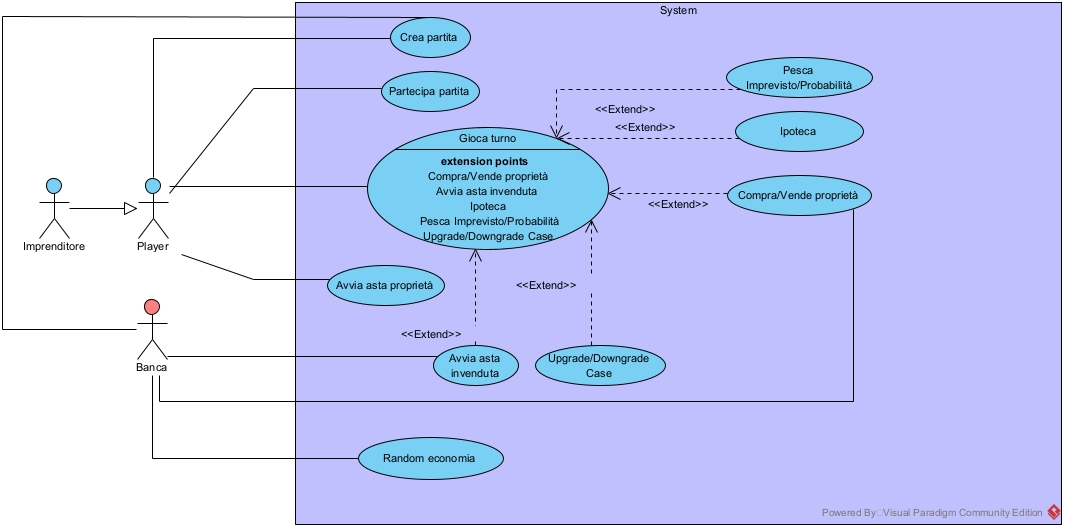
\includegraphics[width=\textwidth]{ModelloCasiDUso}}

\subsection{Modello di dominio}
\href{https://github.com/UnimibSoftEngCourse2022/progetto-monopoly-1-gangoffour2/blob/feat/doc/doc/img/ModelloDiDominio.jpg?raw=true}
	{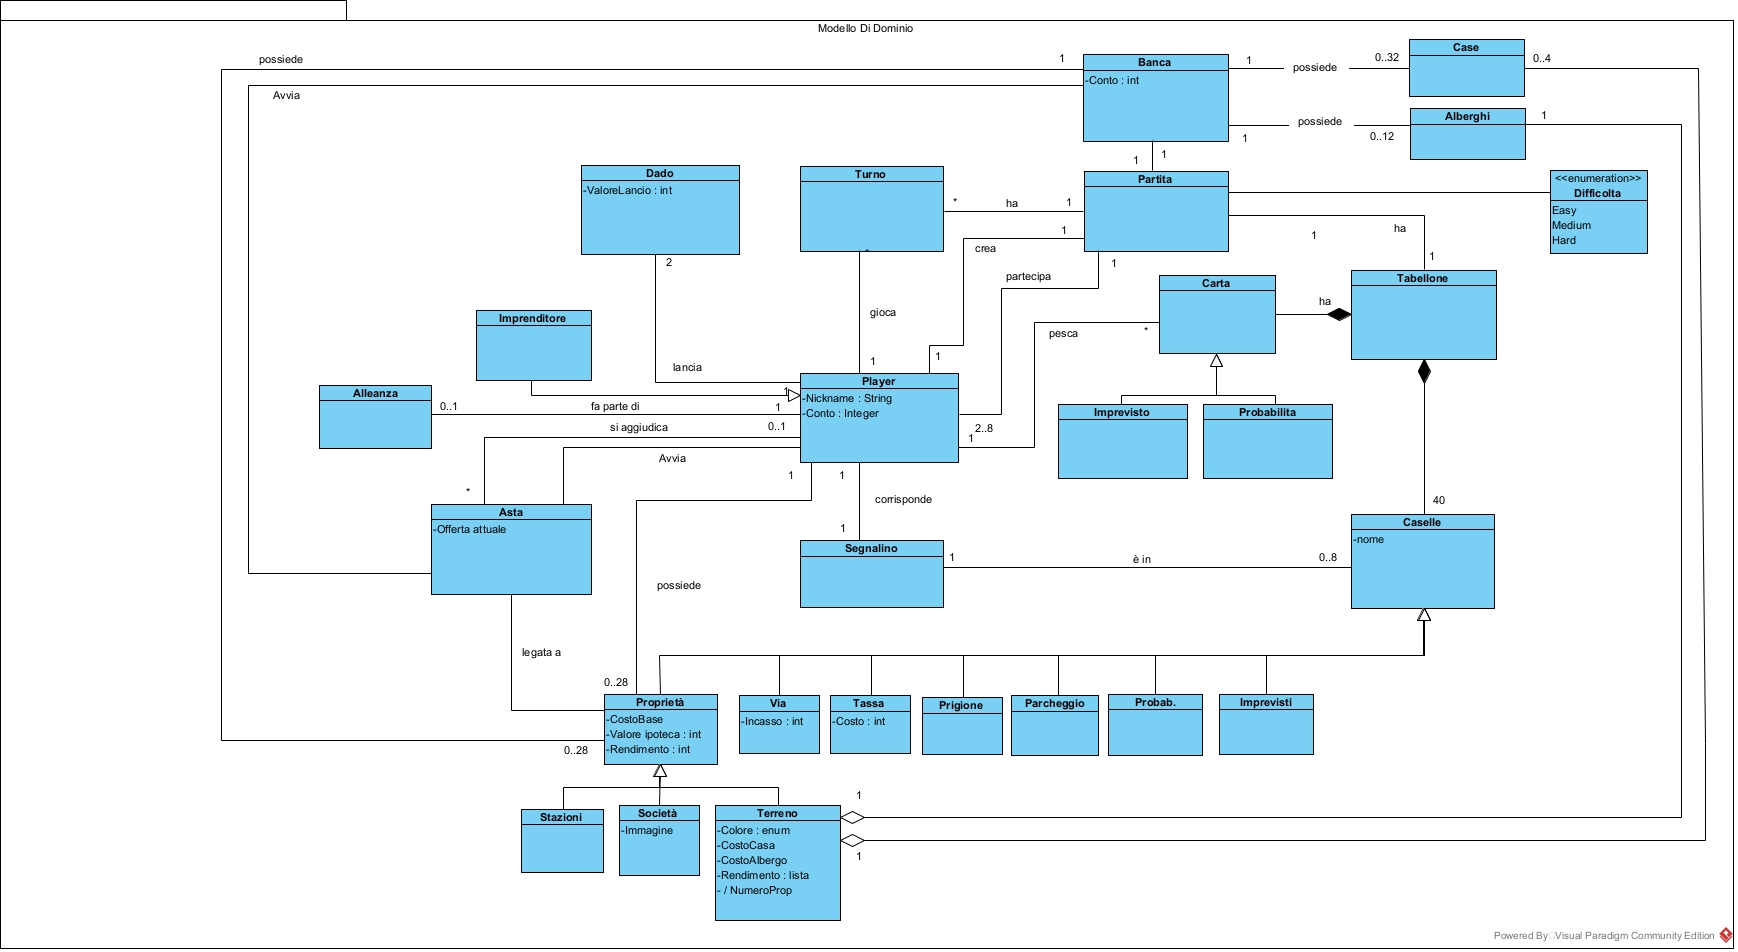
\includegraphics[width=\textwidth]{ModelloDiDominio}}

\subsection{Diagramma delle classi a livello progettazione}
\href{https://github.com/UnimibSoftEngCourse2022/progetto-monopoly-1-gangoffour2/blob/feat/doc/doc/img/DiagrammaDelleClassi.jpg?raw=true}
	{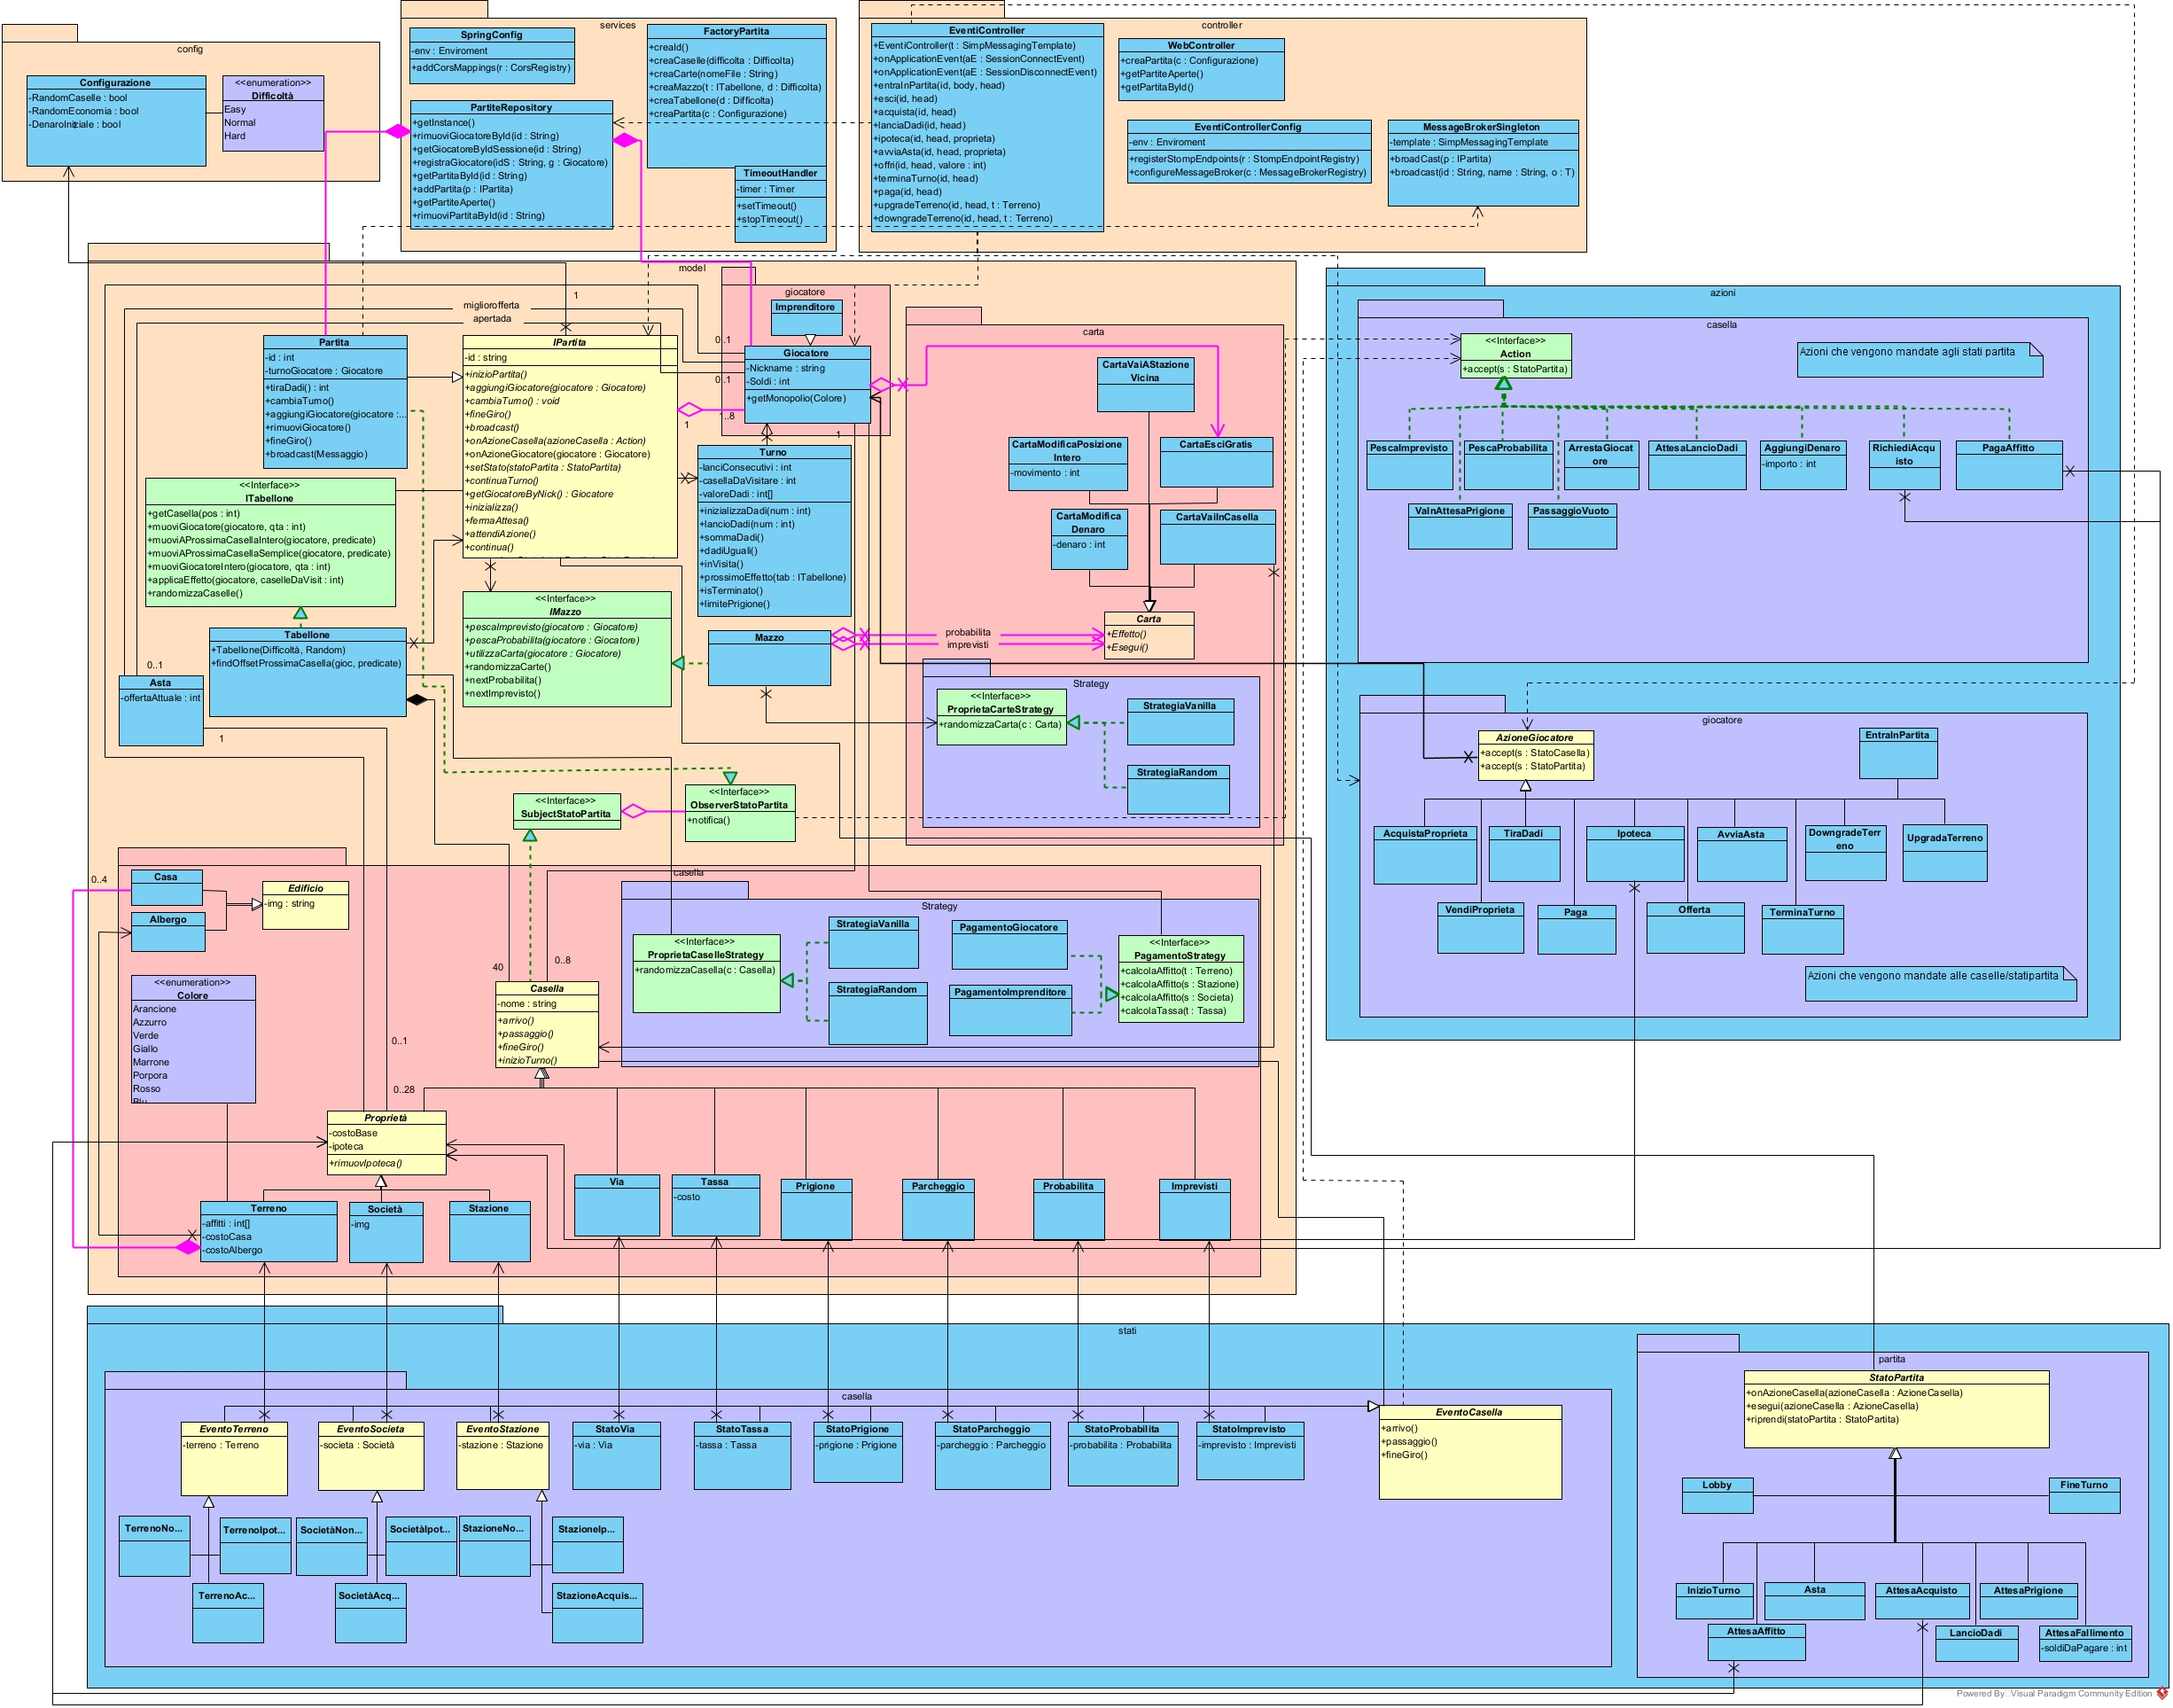
\includegraphics[width=\textwidth]{DiagrammaDelleClassi}}

\subsection{Diagrammi SSD}
\subsubsection{SSD GiocaTurno CasellaProprieta \& Acquisto}
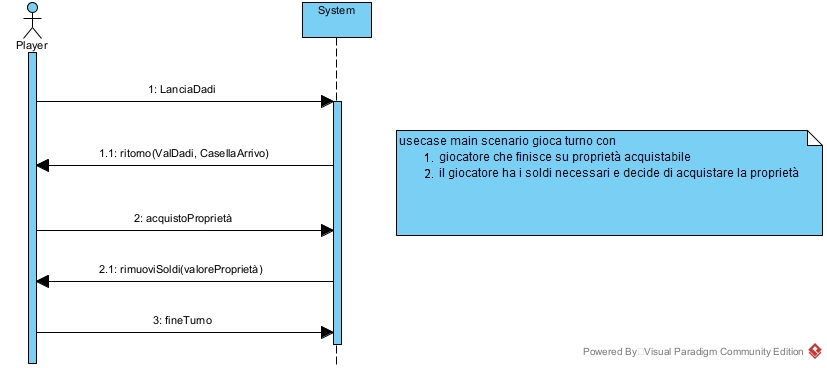
\includegraphics[width=\textwidth]{SSD_GiocaTurno_CasellaProprieta+Acquisto}
\subsubsection{SSD GiocaTurno CasellaProprieta \& No Acquisto}
\includegraphics[width=\textwidth]{SSD_GiocaTurno_CasellaProprietà+NoAcquisto}
\subsubsection{SSD Inizia Asta Terreno invenduto}
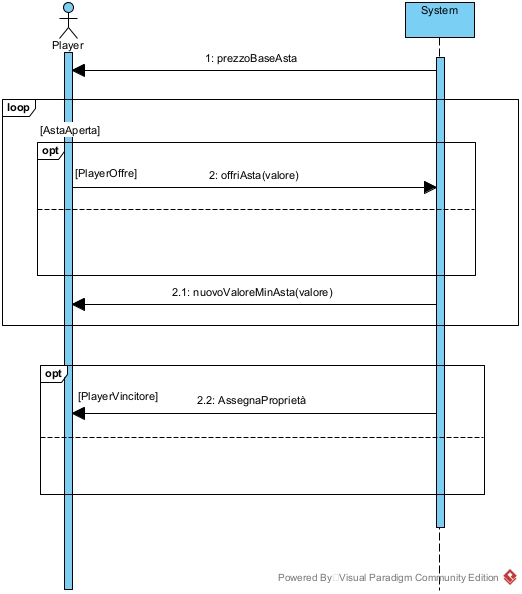
\includegraphics[width=\textwidth]{SSD_IniziaAsta_Invenduta}

\subsection{Diagramma di sequenza}
\href{https://github.com/UnimibSoftEngCourse2022/progetto-monopoly-1-gangoffour2/blob/feat/doc/doc/img/DiagrammaDiSequenzaDiProgettazioneTurnoGiocatore.jpg?raw=true}
	{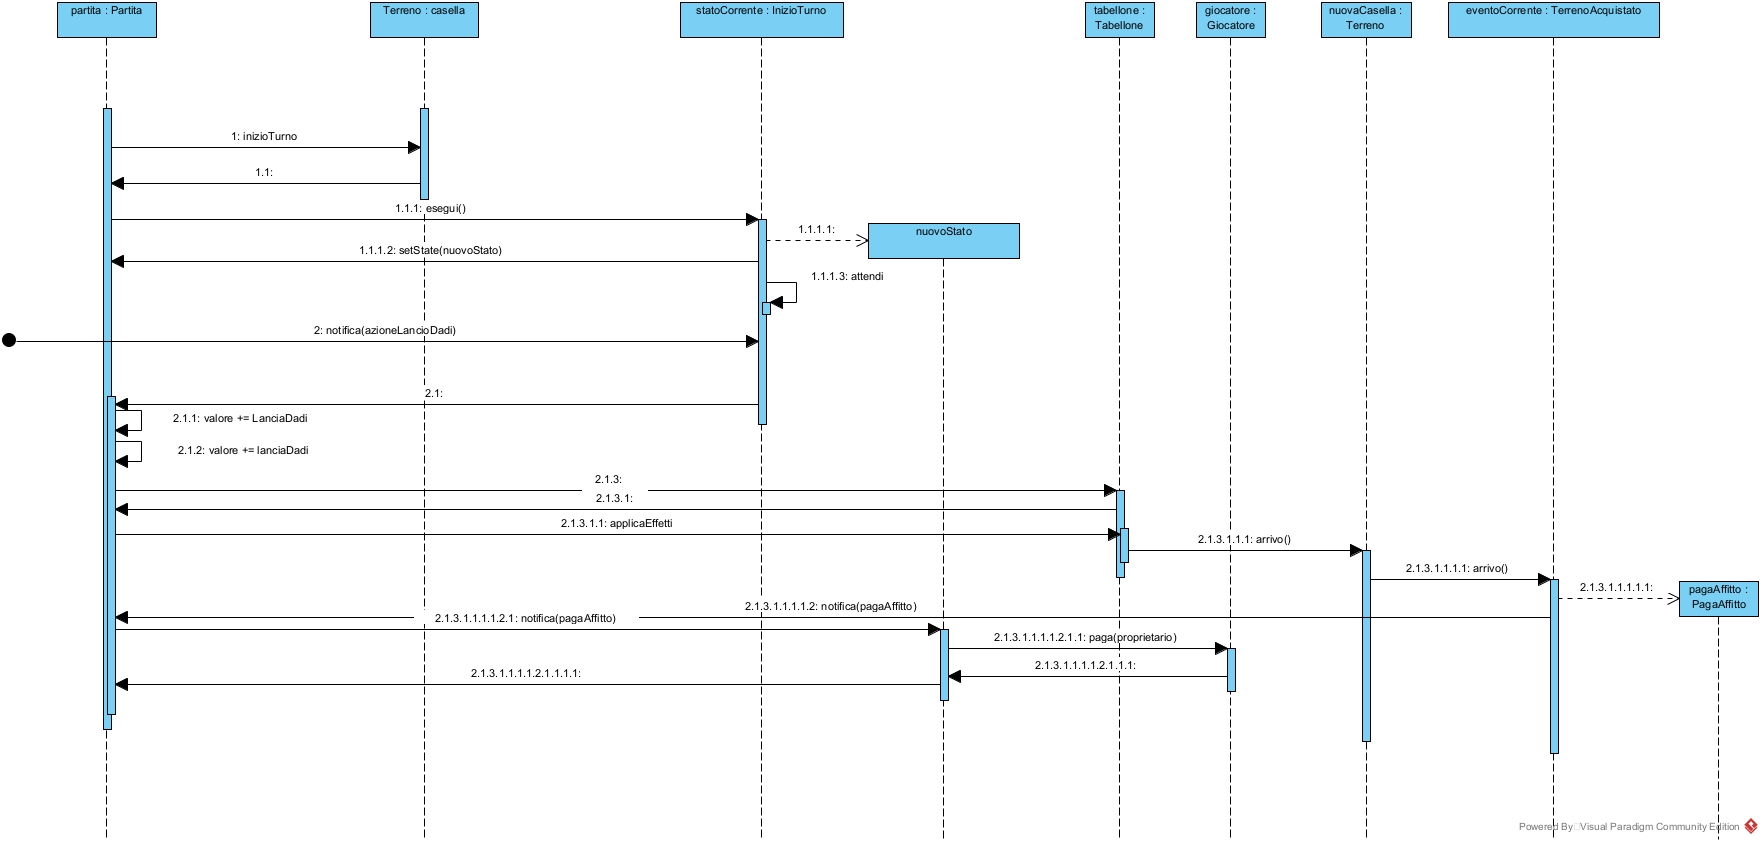
\includegraphics[width=\textwidth]{DiagrammaDiSequenzaDiProgettazioneTurnoGiocatore}}

\subsection{Diagramma Architettura Software}
\href{https://github.com/UnimibSoftEngCourse2022/progetto-monopoly-1-gangoffour2/blob/feat/doc/doc/img/Diagramma_Architettura_Software.jpg?raw=true}
	{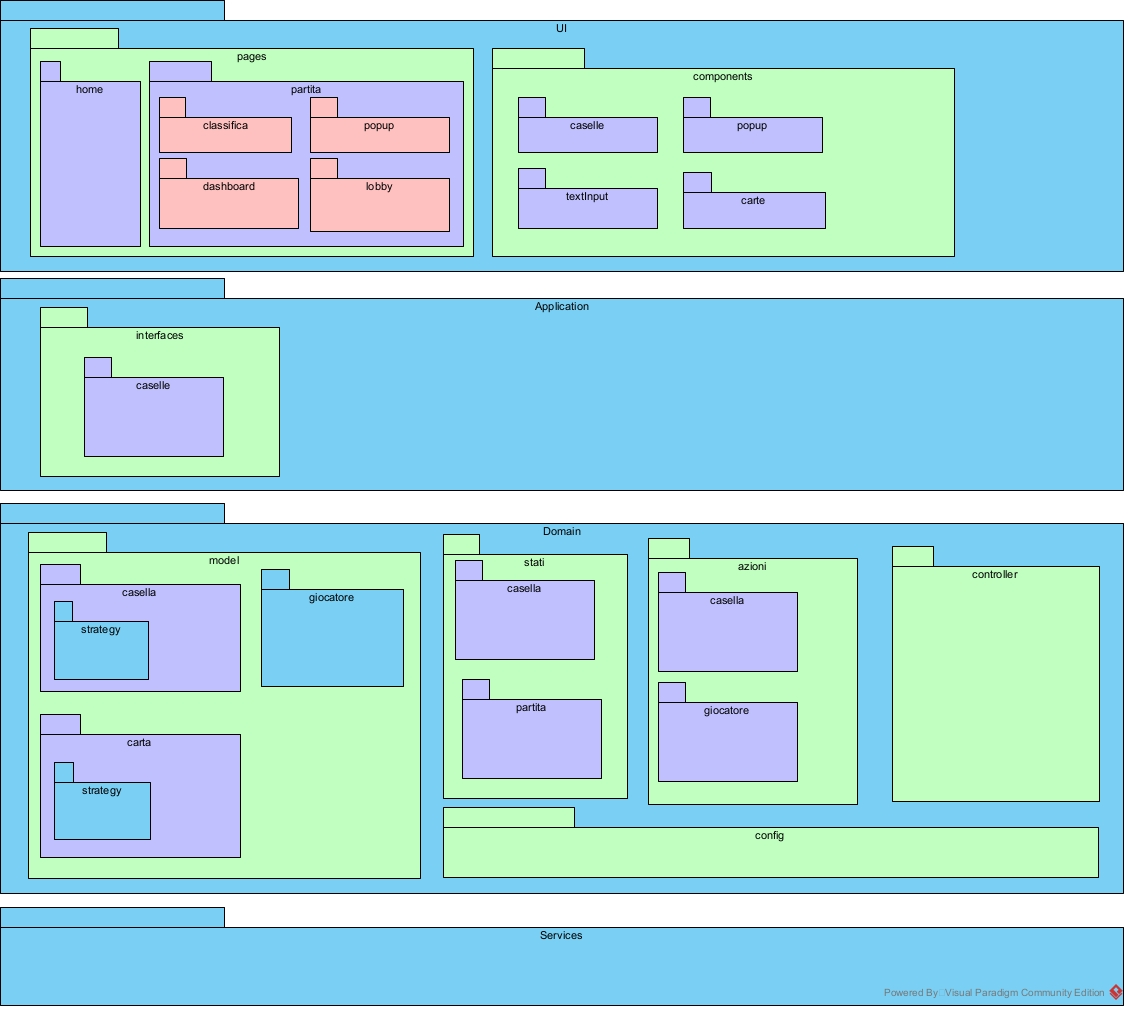
\includegraphics[width=\textwidth]{Diagramma_Architettura_Software}}

\subsection{Diagrammi Stati}
\subsubsection{Diagramma Stati stato partita}
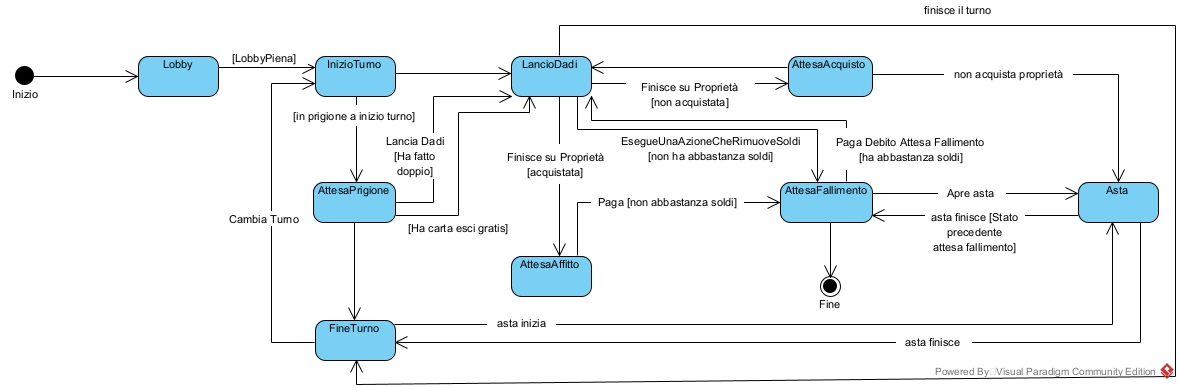
\includegraphics[width=\textwidth]{DiagrammaStatiStatoPartita}
\subsubsection{Diagramma Stati stato terreno}
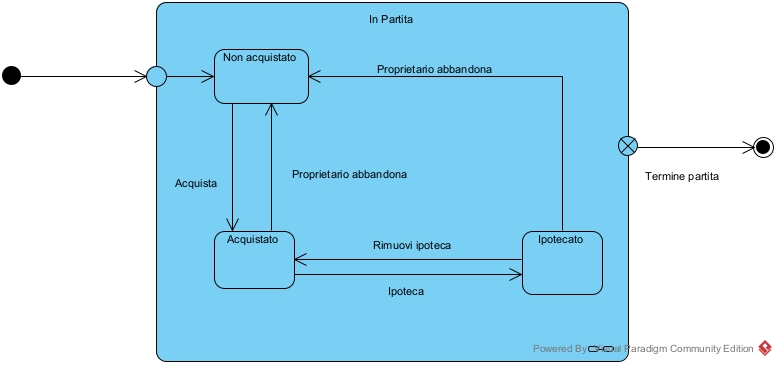
\includegraphics[width=\textwidth]{DiagrammaStatiStatoTerreno}



\section{Progettazione}

\subsection{Tecnologie utilizzate}
\begin{itemize}
	\item \textbf{Server}: per il backend abbiamo voluto utilizzare il framework Spring sia perché complessivamente tutto il team conosce Java e ha avuto esperiente con il framework sia perché ritenuto idoneo allo scopo.


	\item \textbf{Client}: per il frontend è stata principalmente utilizzata la libreria React per costruire l'interfaccia grafica per interagire con il server e costruire dinamicamente il tabellone.
	Sebbene non tutto il team sapesse come utilizzare questa libreria abbiamo convenuto fosse la scelta più ragionevole per l'elevata esperienza di alcuni membri del team che si sono concentrati sullo sviluppo del client.
	
	\item \textbf{Altro}: Sonarqube in locale e Sonarcloud per la CI/CD Pipeline
\end{itemize}


\subsection{Design principles utilizzati}
Nello sviluppo del progetto siamo stati guidati dai principi \textbf{SOLID}:
\begin{itemize}
    \item \textbf{S}ingle-Responsibility principle: classi come Partita, Tabellone e Turno tendono a gestire specifici aspetti del gioco e ad esempio sono state divise concettualmente le caselle, i loro stati e i loro comportamenti.
    
    \item \textbf{O}pen closed principle: il sistema è stato progettando cercando di lasciare la massima possibilità di estenderlo senza andarne a modificare la struttura: ad esempio, è possibile aggiungere un nuovo stato,una nuova casella o nuovi comportamenti senza modificare la struttura principale del sistema.
    
    \item \textbf{L}iskov Substitution Principle: Per fare in modo che la struttura della partita e il suo corretto comportamento non siano influenzati dalla tipologia della singola casella, abbiamo fatto in modo di rendere la gerarchia delle caselle completamente trasparente alla partita.
    
    \item \textbf{I}nterface Segregation Principle: le interfacce utilizzano la keyword default per definire una implementazione base dei metodi che espongono. In questo modo, le classi che implementano tali interfacce sovrascrivono soltanto i metodi che ha effettivamente senso implementare.
    
    \item \textbf{D}ependency Inversion: Per diminuire l'accoppiamento tra classi concrete e aumentare la dipendenza verso classi astratte, abbiamo introdotto varie interfacce che nascondono le implementazioni, tra cui: ITabellone, IPartita, IMazzo.
    \end{itemize}

\subsection{Design patterns utilizzati}
    \begin{itemize}
        \item \textbf{Singleton}: utile per salvare informazioni a cui si può accedere da ogni parte del programma ottenendo sempre la stessa istanza. 
        
        
        \textit{Classi interessate: MessageBrokerSingleton, FactoryPartita, PartiteRepository} 
        
        
        \item \textbf{State}: fondamentale nella struttura del progetto. È stato utilizzato perché il comportamento all'interno di una partita dipende dallo stato di ogni casella, in combinazione con lo stato della partita. Ad esempio, la terminazione su un terreno deve rispondere in modo diverso in base a se è stato acquistato, ipotecato, ecc… \\ La stessa cosa vale per la partita: se la partita sta attendendo che un giocatore paghi l'affitto per un terreno, non è possibile che un altro giocatore lanci i dadi in quel momento. 
        
        \textit{Classi interessate: StatoPartita, Casella} 
        
        
        \item \textbf{Visitor}: Quando una casella notifica un'azione da eseguire alla partita (o meglio, al suo stato), il metodo da eseguire dipende dal tipo concreto di questa azione. \\Per esempio, dato uno stato, il comportamento dipende dal tipo dell'azione generata dalla casella. Inoltre, in questo modo, è possibile aggiungere nuove azioni senza dover modificare la struttura delle classi.
        
        \textit{Classi interessate: AzioniGiocatore, AzioniPartita} 
        
        
        \item \textbf{Strategy}: Utilizzati rispettivamente per per la gestione della randomizzazione di Caselle sul tabellone, di costi delle caselle, di attributi delle carte e definizione di comportamenti diversi per un giocatore di tipo Imprenditore rispetto a uno Standard. 
        \\Il mazzo di carte e il tabellone hanno uno strategy istanziato durante la creazione della partita in base alla difficoltà selezionata. Quando necessario, viene chiamato un metodo su quello strategy che conterrà la logica di gestione specifica per quella difficoltà.
        \\Tutto questo sempre seguendo il principio di apertura ai cambiamenti che in questo permetterà facilmente estendere il software a diversi tipi di strategie legate alle difficoltà di gioco.
        
        \textit{Classi interessate: (Interfaccia)PagamentoStrategy, PagamentoStrategiaGiocatore, PagamentoStrategiaImprenditore, (Interfaccia)ProprietaCaselleStrategy, StrategiaCasellaRandom, StrategiaCasellaVanilla, (Interfaccia)ProprietaCarteStrategy, StrategiaCarteRandom, StrategiaCarteVanilla}
    \end{itemize}

\subsection{Pattern architetturali utilizzati}
    \begin{itemize}
        \item \textbf{Front controller}: utile per fornire un punto di accesso al backend dal client. Classi interessate: EventiController, WebController.
        \item \textbf{Message channel}: utilizzato per gestire le sessioni delle partite con i client. Per fare in modo che tutti i giocatori ricevessero lo stato della partita aggiornato, abbiamo utilizzato un message broker al quale si iscrivono.
    \end{itemize}


\subsection{Problemi incontrati durante la fase di progettazione}
\paragraph{Antipattern strutturali}
Utilizzando il tool Understand, abbiamo notato che la classe Partita aveva molte dipendenze in ingresso e in uscita: questo può essere segno di un antipattern Hub. Per cercare di risolvere il problema, abbiamo aggiunto una classe astratta che viene estesa da partita: In questo modo, abbiamo ridotto le dipendenze in entrata da partita, rendendo visibile solo la classe astratta relativa. Stessa cosa per ITabellone.
\\Invece StatoPartita ha molte dipendenze in entrata, una per ogni tipo di azione 
giocatore/casella. Questo implica che ci potremmo trovare davanti a un Global Butterfly.

\paragraph{}

\end{document}